\section{Experiments}
\label{sec:experiments}


%\begin{figure*}
    %\centering
    %\includegraphics[width=\textwidth]{example-image-a} % Replace with your image file
    %\caption{Caption for the figure.}
    %\label{fig:sample}
%\end{figure*}

%\subsection{Setup}

\noindent \textbf{Setup.} We compare the performance of 
(A)~the quadratic-program-based algorithms
with (B)~the variants of the proportional response algorithms.
The algorithms are implemented in C++.\footnote{The
source codes are available at:
\url{https://github.com/113741090a/Density_Decomposition}}
Since all algorithms use similar data structures and
variables for the allocation variables, for fair comparison, 
we modify existing code to fit into our framework
for the following algorithms from group~(A).
\begin{compactitem}

\item \elist~\cite{DBLP:conf/www/DanischCS17,DBLP:journals/pvldb/SunDCS20} (Algorithm~\ref{algo:elist})

\item \greedypp~\cite{DBLP:conf/www/BoobGPSTWW20} (Algorithm~\ref{algo:greedypp})

\item $\fista^*$~\cite{DBLP:conf/nips/HarbQC22}. This is the variant of Algorithm~\ref{algo:FISTA}
with carefully fine-tuned learning rate.
 %\quan{May mention we use FISTA for hypergraph}.
\end{compactitem}

Based on the experimental findings in~\cite{DBLP:conf/nips/HarbQC22}, 
$\fista^*$ and $\greedypp$ 
demonstrated clear superiority over the basic \fw (Algorithm~\ref{algo:FW-basic}),
which we omit here to avoid redundancy.
On the other hand, their study did not include \elist,
which turns out to have great potential.
On the other hand, we implement the following from group~(B),
where the momentum variants are new algorithms.
\begin{compactitem}

\item $\pr$  (Algorithm~\ref{algo:PR-basic})

\item $\prlin$  (Algorithm~\ref{algo:PR-Momentum}) with linear momentum.

\item $\prexp$  (Algorithm~\ref{algo:PR-Momentum}) with exponential
momentum.

\end{compactitem}






%Describe on high level about the language, the compiler we are using, the machine we are running on...

%A template:  DATASET. We consider 4 datasets in total. The datasets contains up to 11 million edges, as illustrated in \ref{tab:1}. The data is available at snap.stanford.edu.  We tested FW, FISTA, and Proportional response algorithm on these datasets. Then describe details about the implementation, and the machine/system we are running on. We can also discuss how implement the parallel. 


%The data is available at snap.stanford.edu. 

%We tested $4$ algorithms to approximate the Densest Subgraph Decomposition problem. The FISTA based algorithm from~\cite{DBLP:conf/nips/HarbQC22}, the FRANK-WOLFE based algorithm from~\cite{DBLP:conf/www/DanischCS17}, the Proportional Response algorithm~\cite{wu2007proportional, zhang2011proportional} and Proportional Response algorithm combined with momentum. 
%\noindent \textbf{Datasets and Implementation Details.} 

\noindent \textbf{Datasets.}
We use several real-world graphs from~\cite{snapnets}, which contain up to 100 million edges, in Table~\ref{tab:dataset}. 
We describe, in Section~\ref{sec:prelim},
how to interpret
a graph $H = (V, E)$
as a bipartite graph $G = (E, V; \mcal{F})$.
%We denote $|V|= n$ and $|E| = m$; n
Note that
$|\mcal{F}| = 2 |E|$ for a normal graph~$H$.

\noindent \emph{Double Cover.} For a normal graph $H = (V, E)$,
we also consider its \emph{bipartite double cover}
$H^+ = (V, V; \mcal{F})$, where $(u, v) \in \mcal{F}$ \emph{iff}
$\{u, v\} \in E$.  Here, given a subset $S \subseteq V$,
$\mcal{F}[S]$ are the neighbors of $S$ in $G$ 
that are adjacent to only nodes in $S$.  
%Observe that given a normal graph,
Both constructions lead to the same number
of bipartite edges in $\mcal{F}$.


	\noindent \emph{Weighted Directed Graph.} As our framework supports only undirected (hyper)graphs,
	we would first need to transform a directed graph to an undirected graph in a meaningful way.
	
	The dataset wiki-Elec in~\cite{snapnets} is a directed graph indicating Wikipedia administration election data. 	A directed edge from a voter to a candidate
	is labeled with \emph{support} or \emph{no support}.
	
	We produce a weighted undirected graph as follows: every vertex represents a voter, and its weight is the number of times they vote. For any two voters, there is an edge connecting them; the weight of this edge is the number of times they have voted for the same candidate with the same decision.
	%We will run our experiment on this weighted graph. 




\ignore{
\noindent \textbf{Supplementary Material.}
Due to space limit, some figures for the normal graphs
are deferred.  The empirical results for the double covers
lead to the same conclusion as the normal graphs, 
and the corresponding figures are also deferred.
}



\ignore{
For the hypergraph datasets, some graphs are derived from real-world data, while others are generated from normal graphs using the following method: in the hypergraph, the hyperedge and hypernode sets are identical to the vertex set of the original graph. A hyperedge includes a hypernode if and only if there is a link between them in the original graph. Given a vertex set $S$, its closed neighborhood is the subset of $S$ such that all neighbors of the subset are contained within $S$. 
}
%(? from the
%SNAP database [47], and ? from [48]), and one tailored synthetic dataset (used for clarifying an
%important difference between all algorithms) for a total of ? datasets.

\noindent \textbf{Hardware Configuration.}
%Intel(R) Xeon(R) Silver 4114 CPU @ 2.20GHz
We used a Linux server with Intel Xeon(R) Silver 4114 at 2.20 GHz,
with the amount of main memory limited to 57GB. 

%\quan{This setting may not be accurate. To be modified later.}







%This is done after our algorithm partitions the input graph in “sufficiently small” stable subsets. The maximum flow algorithm can then be run in parallel on each such stable subsets

%We compare the following algorithms using various metrics. According to the experimental result in~\cite{DBLP:conf/nips/HarbQC22}, $\fista^*$ and $\greedypp$ is the best two algorithms at that time point. Since they did not include $\elist$ and it is promising, so we include it in our experiment. We also include proportional response based algorithms. 


\ignore{
We tested all the algorithms mentioned in the paper. And compare their performance using various of metrics. 
\quan{Should I mention the details of my implementation? For example, I implemented my own version of all the algorithms. And implementation details about the data structures? How do I implement greedy++? WWW paper does not mention too much about it. NeurIPS paper mentioned it in the appendix. }

}
%All codes are compiled using the \texttt{-O3} optimization level. 

%In the experiments, for each algorithm we will calculate 


\begin{table}[ht]
	\centering
	\caption{Normal Graph Datasets $(V, E)$}
	\label{tab:dataset} % 确保标签放在标题之后
	\begin{tabular}{|l|r|r|l|}
		\hline
		Dataset & $n = |V|$ & $2 |E| = |\mcal{F}|$ & Winner\\
		\hline
		com-amazon & 334,863 & 1,851,744 & $\prexp$\\
		\hline
		dblp-author & 317,080 & 2,099,732 & $\prexp$\\
		\hline
		wiki-Elec & ~6,120 & 2,443,528  & \prexp \\
		\hline
		roadnet-PA & 1,088,092 & 3,083,798 & $\fista^*$\\
		\hline
		roadnet-CA & 1,965,206 & 5,533,214 & $\fista^*$ \\
		\hline
		web-google & 875,713 & 8,644,102 & \prexp \\
		\hline
		cit-patents & 3,774,768 & 33,037,894 & \prexp \\
		\hline
		wiki-topcats & 1,791,489 & 50,888,414 & \prexp\\
		\hline
		orkut & 3,072,441 & 234,370,166  & \prexp \\
		\hline
	\end{tabular}
\end{table}

	

\ignore{
\begin{table}[ht]
	\centering
	\caption{Hypergraph Dataset}
	\label{tab:hyperdata} % 确保标签放在标题之后
	\begin{tabular}{|l|l|l|l|}
		\hline
		Dataset & Vertices & Edges & Source \\
		\hline
		wiki-Elec & 7K & 100k & [47] \\
		\hline
	\end{tabular}
\end{table}
}

\subsection{Approximation Quality vs Number of Iterations}

To measure the approximation accuracy,
we compute the exact density vector~$\rho^*$
for each graph.

\noindent \textbf{Exact Decomposition.}
The method described in \cite{DBLP:conf/www/DanischCS17} is already scalable for large real-world graphs. Initially, they use an iterative method (such as \elist) to obtain an approximate density vector. Subsequently, heuristic methods are applied to partition the graph into stable blocks, as defined in Definition~\ref{defn:stable-block}. Once the stable blocks are sufficiently small, $\mathsf{AtomicOrSplit}$ (Algorithm~\ref{algo:maxflow}) is employed to complete the decomposition.

In practice, 100 to 500 iterations of the iterative algorithms typically yield sufficiently accurate density vectors, enabling the heuristic methods to compute the exact density decompositions. Nevertheless, in our experiments, we compare different iterative algorithms beyond 1000 iterations to examine their convergence behavior.

In Figure~\ref{fig:accuracy_iteration_normal_1} and Figure~\ref{fig:errors_hyper}, we show, as the number $T$ of iterations increases, how the following approximation metrics
change for each method.

\begin{compactitem}

\item \emph{Global Error} (Definition~\ref{defn:error}).

\item  \emph{Local Error} (Definition~\ref{defn:error}). 

\item \emph{Number of Inversions} (Definition~\ref{def:order1}).
Unlike the previous two notions, 
the number of inversions
will theoretically reach~0.  
%We use this to determine the number of iterations to run for each graph.

\end{compactitem}


\ignore{

In this subsection we test the relationship between the approximate quality and the number of iterations. There are various metrics to evaluate the approximate quality, here given an approximate density vector $\hat{\rho}$, we mainly focus on its \emph{Global Error} (Definition~\ref{defn:error}), \emph{Local Error}(Definition~\ref{defn:error}) and \emph{Number of Inversions}(Definition~\ref{def:order1}). 



In the experiment, since the exact density vector is available, we set the number of iterations $T$ to be the minimum number of iterations such that at least one algorithm reaches $0$ number of inversions. Because if this happens, then there is no need to continue the iterative algorithms, using the heuristic method in \cite{DBLP:conf/www/DanischCS17} can already output the correct density decomposition efficiently. 

For every two iterations, we calculate the approximate density vector and evaluate the corresponding metrics. In each figure within this subsection, the x-axis represents the number of iterations, while the y-axis may depict various metrics. Separate figures are created for each metric using datasets from Tables~\ref{tab:dataset} and~\ref{tab:hyperdata}.

%In figure~\ref{fig:global_error_hyper}, the input instances are more general and may contain a hyperedge $e$ with large $|e|$. 

\noindent \textbf{Global Error. }Figure~\ref{fig:global_error} and Figure~\ref{fig:global_error_hyper} shows the relationship between the number of iterations and the global error for different graphs. In figure~\ref{fig:global_error}, the input instances are from Table~\ref{tab:dataset}. 
In figure~\ref{fig:global_error_hyper}, the input instances are from Table~\ref{tab:hyperdata}. 

\noindent \textbf{Local Error. }Figure~\ref{fig:local_error} and Figure~\ref{fig:local_error_hyper} shows the relationship between the number of iterations and the global error for different graphs. In figure~\ref{fig:local_error}, the input instances are from Table~\ref{tab:dataset}. 
In figure~\ref{fig:local_error_hyper}, the input instances are from Table~\ref{tab:hyperdata}. 

\noindent \textbf{Number of Inversions. }Figure~\ref{fig:inv} and Figure~\ref{fig:inv_hyper} shows the relationship between the number of iterations and the global error for different graphs. In figure~\ref{fig:inv}, the input instances are from Table~\ref{tab:dataset}. 
In figure~\ref{fig:inv_hyper}, the input instances are from Table~\ref{tab:hyperdata}. 

}

\noindent \textbf{Interesting Empirical Observations.}
In general, the three approximation metrics are consistent with each other, where in some graphs, the number of inversions can reach 0. While the global error decreases smoothly with the number of iterations, both the local error and the number of iterations exhibit some fluctuations despite the overall decreasing trend.
Below are general comparisons between the different methods.

\begin{compactitem}

\item The new algorithm $\prexp$ is the clear winner 
in many graphs, offering an improvement margin of several orders of magnitude compared to the closest competitor.

We observe that in roadnet-PA and roadnet-CA, $\fista^*$ performs slightly better 
than $\prexp$ in terms of global and local error, and can achieve zero number of inversions.  However, on graphs where $\fista^*$ is not the winner, its performance can be significantly worse than other
methods in group~(A) such as \elist.

Hence, for very large graphs (cit-patents, wiki-topcats and orkut), we only compare $\prexp$, $\fista^*$
and \elist, the last of which runs the fastest.


\item Without momentum, the basic \pr method has a similar behavior as
the quadratic-program-based methods in group~(A).

The algorithm $\prlin$ with linear momentum
initially has a similar behavior as $\prexp$.
However, after a small number of iterations,
$\prlin$ seems to offer no further progress on the accuracy.

\item 
As corroborated in the previous study~\cite{DBLP:conf/nips/HarbQC22},
the quadratic-program-based methods in group~(A) exhibit similar behavior. 

\item It is somewhat surprising that, in most graphs, $\greedypp$ outperforms \elist slightly, even though \elist intuitively distributes the edge weights among nodes more evenly.

%\item 
%Typically, $\fista^*$ does not perform well initially, but it improves rapidly as the number of iterations increases.


\end{compactitem}


\ignore{

We observe that  Usually, $\fista^*$ is not good initially, but improves fast when the number of iterations is large. On the contrary, $\prlin$ improves very fast initially, but then improves very slowly when the number of iterations is large. The behavior of $\prlin$ and $\prexp$ are very similar initially. The performance of $\elist$ and $\greedypp$ are similar. In most cases, $\greedypp$ is better than $\elist$. The performance $\pr$ is not very good for datasets in Table~\ref{tab:dataset}. However, its performance is very good for datasets in Table~\ref{tab:hyperdata}, especially for local error and the number of inversions.
}


\subsection{Running Time and Simulated Wall Clock Time}


We evaluate the running times of the different algorithms across various input sizes.
Because all methods are iterative and each algorithm repeats the same computations
in every iteration, we measure the wall clock time for 100 iterations in each setting,
as opposed to the time for the whole execution.  Here are the advantages:

\begin{compactitem}
\item Focusing on the time for a specific but sufficient number of iterations allows for a more controlled environment to measure the running time.

\item Running the whole execution may be more susceptible to occasional irregularities caused by system noise, background processes, or other transient factors.
\end{compactitem}


\noindent \textbf{Measurements.}  For each algorithm on each graph,
we measure the time for 100 iterations.  We repeat the experiment to collect 10 data points.
It turns out the population standard deviation is within $1 \sim 2 \%$ of the average.
Hence, in the left subfigures of Figure~\ref{fig:time_mem}, we show
the average time per iteration against the size of the graph, as measured by $|\mcal{F}|$.
We omit the standard deviation bars as they would appear negligible in the plot.
%Each algorithm is represented by a separate bar in the bar chart, with error bars indicating the variance in running times. 

\noindent \textbf{Running Times Results.}
In terms of
per iteration, \greedypp is the slowest, while \elist is the fastest.
However, the running times are more meaningful when they
are interpreted together with the approximation quality.
Combining the data from Figures~\ref{fig:accuracy_iteration_normal_1} and~\ref{fig:time_mem_normal},
we simulate the wall clock time in Figure~\ref{fig:accuracy_time_normal_graphs_1} for normal graphs,
by multiplying the iteration~$t$ with the average time per iteration. Similarly, we simulate the wall clock time in Figure~\ref{fig:errors_hyper_time} for double covers. 

In general, the method $\prexp$ is still better than the closest competitors \elist and $\fista^*$ most of the time.
For instance, at the time when $\fista^*$ or \elist finishes,
we see that \prexp has a better approximation accuracy in most graphs.

\ignore{

\begin{compactitem}
\item  
\end{compactitem}

}





\ignore{



 The main steps of our experimental setup are as follows:

\begin{itemize}
	\item \textbf{Input Size Variation:} The input sizes were varied from small to large, specifically: $10, 50, 100, 500, 1000, 5000, \text{ and } 2\cdot 10^8$. \quan{To be modified..}
	\item \textbf{Iterations:} Each algorithm was executed $100$ times for each input size to ensure the reliability and stability of the results.
	\item \textbf{Data Collection:} The running time for each execution was recorded, and the average, variance running time over $100$ iterations was computed.
	%\item \textbf{Error Analysis:} The standard error for each algorithm at each input size was calculated and represented using error bars in the results graph.
\end{itemize}

The results of the experiment are illustrated in Figure \ref{fig:results}, where the datasets are ordered by graph size on the x-axis and the y-axis represents the corresponding running times. Each algorithm is represented by a separate bar in the bar chart, with error bars indicating the variance in running times. 

\quan{Describe the observations.}

}
%For each graph, we run $100$ iterations and calculate the average run-time. Then draw the relationship between the run-time and the size of the graph. The size of the graph is evaluated by the sum of the degrees. We also draw error bars in the figures. 
%We examine the average run-time per iteration after $T$ iterations. 


%\subsection{Densities}
%We ran all the algorithms for a number of iterations, and monitored the maximum density reached by the algorithm until iteration $t$. 


 




%such that the number of inversions drop to $0$ for at least one algorithm. 


\ignore{

\subsection{Approximate Quality vs (Simulated) Wall Clock Time}
Apart from the number of iterations, we also evaluate the relationship between the approximate quality and the wall clock time. 

Since wall clock time may not be stable, we will compute the average running time for each algorithm across a set of representative graphs after a certain number of iterations. Subsequently, at iteration $t$, we will approximate the wall clock time by multiplying $t$ with the previously determined average time. This approach is designed to mitigate stability concerns and provide a more consistent estimation of performance. 

\noindent \textbf{Global Error. }Figure~\ref{fig:global_error_time} and Figure~\ref{fig:global_error_hyper_time} shows the relationship between the number of iterations and the global error for different graphs. In figure~\ref{fig:global_error_time}, the input instances are from Table~\ref{tab:dataset}. 
In figure~\ref{fig:global_error_hyper_time}, the input instances are from Table~\ref{tab:hyperdata}. 

\noindent \textbf{Local Error. }Figure~\ref{fig:local_error_time} and Figure~\ref{fig:local_error_hyper_time} shows the relationship between the number of iterations and the global error for different graphs. In figure~\ref{fig:local_error_time}, the input instances are from Table~\ref{tab:dataset}. 
In figure~\ref{fig:local_error_hyper_time}, the input instances are from Table~\ref{tab:hyperdata}. 

\noindent \textbf{Number of Inversions. }Figure~\ref{fig:inv_time} and Figure~\ref{fig:inv_hyper_time} shows the relationship between the number of iterations and the global error for different graphs. In figure~\ref{fig:inv_time}, the input instances are from Table~\ref{tab:dataset}. 
In figure~\ref{fig:inv_hyper_time}, the input instances are from Table~\ref{tab:hyperdata}. 

}




%%%%%%%%%%%%%%%%%%%%%%%%%%%%
%
% Accuracy vs Iterations: Normal Graph I
% Group the figures into one
\begin{figure*}[htbp]
	\centering
	\begin{subfigure}[b]{\textwidth}
		\centering
	% ???????????
	\begin{minipage}[b]{0.05\textwidth}
		\centering
        \raisebox{1.5cm}{
	\tiny % ????????????
	\renewcommand{\baselinestretch}{0.8}\selectfont % ?????
	\begin{tabular}{c}
		F \\
		A \\
		C \\
		E \\
		B  \\
		O \\
		O \\
		K
	\end{tabular}
	}
		%\raisebox{1.5cm}{\rotatebox{90}{\textbf{Main Title}}} % ?????????
	\end{minipage}%
	% ?????
	\begin{minipage}[b]{0.3\textwidth}
		\centering
		\caption*{Global Error} % ???
		\includegraphics[width=\textwidth]{images/facebook/figures_normal/Absolute_Error_vs_T.png} % ?????????
		
	\end{minipage}%
	% ?????
	\begin{minipage}[b]{0.3\textwidth}
		\centering
		\caption*{Local Error} % ???
		\includegraphics[width=\textwidth]{images/facebook/figures_normal/Multiplicative_Error_vs_T.png} % ?????????
		
	\end{minipage}%
	% ?????
	\begin{minipage}[b]{0.3\textwidth}
		\centering
		\caption*{Number of Inversions} % ???
		\includegraphics[width=\textwidth]{images/facebook/figures_normal/inv_vs_T.png} % ?????????
	\end{minipage}
\end{subfigure}

%%%%%%%%%%
%%%%%%%%%
\caption{Approximation Quality vs Number of Iterations: Selected Normal Graphs}
\label{fig:accuracy_iteration_normal_1}
\end{figure*}




%%%%%%%%%%%%%%%%%%%%%%%%%%%%%%
%%%%%%%%%%%%%%%%%%%%%%%%%%%%%

\begin{figure*}[htbp]
\centering
\begin{subfigure}[b]{\textwidth}
	\centering
\begin{minipage}[b]{0.3\textwidth}
			\centering
			%\caption*{Time-Normal Graph} % ???
			\includegraphics[width=\textwidth]{images/time_mem/time_normal/time_comparison_table.png} % ?????????
			
		\end{minipage}%
		% ?????
		\begin{minipage}[b]{0.3\textwidth}
			\centering
			%\caption*{Memory-Normal Graph} % ???
			\includegraphics[width=\textwidth]{images/time_mem/mem_normal/memory_usage_table.png} % ?????????
			
		\end{minipage}%

		\caption{Running Time and Memory Usage vs Graph Size on Normal Graphs}
\label{fig:time_mem_normal}
\end{subfigure}
\begin{subfigure}[b]{\textwidth}
	\centering
	\begin{minipage}[b]{0.3\textwidth}
	\centering
	%\caption*{Time-Hyper Graph} % ???
	\includegraphics[width=\textwidth]{images/time_mem/time_hyper/time_comparison_table.png} % ?????????
	
\end{minipage}%
% ?????
\begin{minipage}[b]{0.3\textwidth}
	\centering
	%\caption*{Memory-Hyper Graph} % ???
	\includegraphics[width=\textwidth]{images/time_mem/mem_hyper/memory_usage_table.png} % ?????????
\end{minipage}%
	\caption{Running Time and Memory Usage vs Graph Size on Double Covers}
\label{fig:time_mem_double}
\end{subfigure}
\caption{}
\label{fig:time_mem}
\end{figure*}



%%%%%%%%%%%%%
%
%  Simulated Wall Clock Time
% Group the figures into one
\begin{figure*}[htbp]
	\centering
	\begin{subfigure}[b]{\textwidth}
		\centering
		% ???????????
		\begin{minipage}[b]{0.05\textwidth}
			\centering
			\raisebox{1.5cm}{
				\tiny % ????????????
				\renewcommand{\baselinestretch}{0.8}\selectfont % ?????
				\begin{tabular}{c}
					F \\
					A \\
					C \\
					E \\
					B  \\
					O \\
					O \\
					K
				\end{tabular}
			}
			%\raisebox{1.5cm}{\rotatebox{90}{\textbf{Main Title}}} % ?????????
		\end{minipage}%
		% ?????
		\begin{minipage}[b]{0.3\textwidth}
			\centering
			\caption*{Global Error} % ???
			\includegraphics[width=\textwidth]{images/facebook/figures_normal/Absolute_Error_vs_Time.png} % ?????????
			
		\end{minipage}%
		% ?????
		\begin{minipage}[b]{0.3\textwidth}
			\centering
			\includegraphics[width=\textwidth]{images/facebook/figures_normal/Multiplicative_Error_vs_Time.png} % ?????????
			
		\end{minipage}%
		% ?????
		\begin{minipage}[b]{0.3\textwidth}
			\centering
			\caption*{Number of Inversions} % ???
			\includegraphics[width=\textwidth]{images/facebook/figures_normal/inv_vs_Time.png} % ?????????
		\end{minipage}
	\end{subfigure}
	%%
	\caption{Approximation Quality vs Simulated Wall Clock Time: Selected Normal Graphs}
	\label{fig:accuracy_time_normal_graphs_1}
\end{figure*}

%%%%%%%%%%%%%%%%%%%%%%%%%%%
% Group the figures into one


\begin{figure*}[bp]
	%\begin{figure*}[H]
	\centering
	\begin{subfigure}[b]{\textwidth}
		\centering
		% ???????????
		\begin{minipage}[b]{0.05\textwidth}
			\centering
			\raisebox{1.5cm}{
				\tiny % ????????????
				\renewcommand{\baselinestretch}{0.8}\selectfont % ?????
				\begin{tabular}{c}
					F \\
					A \\
					C \\
					E \\
					B \\
					O \\
					O \\
					K
				\end{tabular}
			}
			%\raisebox{1.5cm}{\rotatebox{90}{\textbf{Main Title}}} % ?????????
		\end{minipage}%
		% ?????
		\begin{minipage}[b]{0.3\textwidth}
			\centering
			\includegraphics[width=\textwidth]{images/parameters/facebook/figures/Absolute_Error_vs_T.png} % ?????????
			
		\end{minipage}%
		% ?????
		\begin{minipage}[b]{0.3\textwidth}
			\centering
			
			\includegraphics[width=\textwidth]{images/parameters/facebook/figures/Multiplicative_Error_vs_T.png} % ?????????
			
		\end{minipage}%
		% ?????
		\begin{minipage}[b]{0.3\textwidth}
			\centering
			
			\includegraphics[width=\textwidth]{images/parameters/facebook/figures/inv_vs_T.png} % ?????????
		\end{minipage}
	\end{subfigure}
	%%%%%
	\caption{Approximation Quality vs Number of Iterations for \prexp with Different $C$ in 
		$\gamma_t = 1 - \frac{C}{t+C}$, for $C = 1, 2, \ldots, 6$
	}
	\label{fig:parameter_normal_graphs}
\end{figure*}




%%%%%%%%%%%%%
%%%%%%%%%%%%


% Group the figures into one
\begin{figure*}[htbp]
	\centering

		\begin{subfigure}[b]{\textwidth}
			\centering
			% ???????????
			\begin{minipage}[b]{0.05\textwidth}
				\centering
				\raisebox{1.5cm}{
					\tiny % ????????????
					\renewcommand{\baselinestretch}{0.8}\selectfont % ?????
					\begin{tabular}{c}
						F \\
						A \\
						C \\
						E \\
						B  \\
						O \\
						O \\
						K
					\end{tabular}
				}
				%\raisebox{1.5cm}{\rotatebox{90}{\textbf{Main Title}}} % ?????????
			\end{minipage}%
			% ?????
			\begin{minipage}[b]{0.3\textwidth}
				\centering
				\caption*{Global Error} % ???
				\includegraphics[width=\textwidth]{images/facebook/figures_hyper/Absolute_Error_vs_T.png} % ?????????
				
			\end{minipage}%
			% ?????
			\begin{minipage}[b]{0.3\textwidth}
				\centering
				\caption*{Local Error} % ???
				\includegraphics[width=\textwidth]{images/facebook/figures_hyper/Multiplicative_Error_vs_T.png} % ?????????
				
			\end{minipage}%
			% ?????
			\begin{minipage}[b]{0.3\textwidth}
				\centering
				\caption*{Number of Inversions} % ???
				\includegraphics[width=\textwidth]{images/facebook/figures_hyper/inv_vs_T.png} % ?????????
			\end{minipage}
		\end{subfigure}
	
	%
	\caption{Approximation Quality vs Number of Iterations: Selected Double Covers}
	\label{fig:errors_hyper}
\end{figure*}







% Group the figures into one
\begin{figure*}[htbp]
	\centering

		\begin{subfigure}[b]{\textwidth}
			\centering
			% ???????????
			\begin{minipage}[b]{0.05\textwidth}
				\centering
				\raisebox{1.5cm}{
					\tiny % ????????????
					\renewcommand{\baselinestretch}{0.8}\selectfont % ?????
					\begin{tabular}{c}
						F \\
						A \\
						C \\
						E \\
						B  \\
						O \\
						O \\
						K
					\end{tabular}
				}
				%\raisebox{1.5cm}{\rotatebox{90}{\textbf{Main Title}}} % ?????????
			\end{minipage}%
			% ?????
			\begin{minipage}[b]{0.3\textwidth}
				\centering
				\caption*{Global Error} % ???
				\includegraphics[width=\textwidth]{images/facebook/figures_hyper/Absolute_Error_vs_Time.png} % ?????????
				
			\end{minipage}%
			% ?????
			\begin{minipage}[b]{0.3\textwidth}
				\centering
				\caption*{Local Error} % ???
				\includegraphics[width=\textwidth]{images/facebook/figures_hyper/Multiplicative_Error_vs_Time.png} % ?????????
				
			\end{minipage}%
			% ?????
			\begin{minipage}[b]{0.3\textwidth}
				\centering
				\caption*{Number of Inversions} % ???
				\includegraphics[width=\textwidth]{images/facebook/figures_hyper/inv_vs_Time.png} % ?????????
			\end{minipage}
		\end{subfigure}
	%
	\caption{Approximation Quality vs Simulated Wall Clock Time: Selected Double Covers}
	\label{fig:errors_hyper_time}
\end{figure*}



\subsection{Memory Usage}

We evaluate the maximum memory usage of the algorithms by reading \texttt{/proc/self/status}. 
The right subfigures in Figure~\ref{fig:time_mem} report the maximum memory usage of each algorithm
against the graph size in terms of $\mcal{F}$.
As expected, the memory usage for all algorithms exhibits a linear dependence on the size $\mcal{F}$ because they use the same graph data structure and keep the same weight allocation variables. The slight difference is due to auxiliary data structures used for greedy choices in each algorithm.


\subsection{Momentum Parameters}
When we run $\prexp$, 
we have so far followed the conventional choice of using
the momentum parameter
 $\gamma_t = 1 - \frac{3}{t+3}$.
Similar to \cite{DBLP:conf/nips/HarbQC22}, 
we next investigate $\gamma_t = 1 - \frac{C}{t+C}$
for different choices of $C$. In this experiment, we run $\prexp$ with difference values of $C= 1, 2, 3, 4, 5, 6$, and investigate the relationship between approximation quality and the number of iterations. See Figure~\ref{fig:parameter_normal_graphs} for the results. 


\noindent \textbf{Observations.} We observe that for
all approximation notions, the quality of approximation
improves when $C$ increases from 1 to 4.
In terms of local and global errors, $C = 4$ yields the best results, with only minor differences compared to $C = 5$ and $C = 6$. However, regarding the number of inversions, $C = 5$ and $C = 6$ perform better than $C = 4$.  Hence, it may be interesting to investigate further
if $C=4$ has any theoretical advantage over the conventional choice of $C=3$.


%We find that $C=4,5,6$ is better than $C = 1, 2, 3$ in all measurements. 
%we try $C = 1, 2, 3, 4, 5, 6$ and investigate the effect of difference choices of $C$. 



% Your text above the figure
%\lipsum[1-2] % Placeholder text
%\suppressfloats[t] % 阻止顶部浮动体堆积

%\begin{figure}[!h] % 强制优先处理
\ignore{
\begin{figure*}[bp]
%\begin{figure*}[H]
	\centering
	\begin{subfigure}[b]{\textwidth}
		\centering
		% ???????????
		\begin{minipage}[b]{0.05\textwidth}
			\centering
			\raisebox{1.5cm}{
				\tiny % ????????????
				\renewcommand{\baselinestretch}{0.8}\selectfont % ?????
				\begin{tabular}{c}
					W \\
					E \\
					B \\
					\vrule\\
					G  \\
					O  \\
					O  \\
					G  \\
					L  \\
					E  \\
				\end{tabular}
			}
			%\raisebox{1.5cm}{\rotatebox{90}{\textbf{Main Title}}} % ?????????
		\end{minipage}%
		% ?????
		\begin{minipage}[b]{0.3\textwidth}
			\centering
			\includegraphics[width=\textwidth]{images/parameters/web-google/Absolute_Error_vs_T.png} % ?????????
			
		\end{minipage}%
		% ?????
		\begin{minipage}[b]{0.3\textwidth}
			\centering
			
			\includegraphics[width=\textwidth]{images/parameters/web-google/Multiplicative_Error_vs_T.png} % ?????????
			
		\end{minipage}%
		% ?????
		\begin{minipage}[b]{0.3\textwidth}
			\centering
			
			\includegraphics[width=\textwidth]{images/parameters/web-google/inv_vs_T.png} % ?????????
		\end{minipage}
	\end{subfigure}
	%CATS
	\begin{subfigure}[b]{\textwidth}
		\centering
		% ???????????
		\begin{minipage}[b]{0.05\textwidth}
			\centering
			\raisebox{1.5cm}{
				\tiny % ????????????
				\renewcommand{\baselinestretch}{0.8}\selectfont % ?????
				\begin{tabular}{c}
					W \\
					I \\
					K \\
					I \\
					\vrule\\
					T\\
					O\\
					P\\
					C\\
					A\\
					T\\
					S
				\end{tabular}
			}
			%\raisebox{1.5cm}{\rotatebox{90}{\textbf{Main Title}}} % ?????????
		\end{minipage}%
		% ?????
		\begin{minipage}[b]{0.3\textwidth}
			\centering
			\includegraphics[width=\textwidth]{images/parameters/wiki-cats/Absolute_Error_vs_T.png} % ?????????
			
		\end{minipage}%
		% ?????
		\begin{minipage}[b]{0.3\textwidth}
			\centering
			
			\includegraphics[width=\textwidth]{images/parameters/wiki-cats/Multiplicative_Error_vs_T.png} % ?????????
			
		\end{minipage}%
		% ?????
		\begin{minipage}[b]{0.3\textwidth}
			\centering
			
			\includegraphics[width=\textwidth]{images/parameters/wiki-cats/inv_vs_T.png} % ?????????
		\end{minipage}
	\end{subfigure}
%%%%%
	\caption{Approximation Quality vs Number of Iterations for \prexp with Different $C$ in 
	$\gamma_t = 1 - \frac{C}{t+C}$, for $C = 1, 2, \ldots, 6$
	}
	\label{fig:parameter_normal_graphs}
\end{figure*}

}


%of the algorithms. The datasets are sorted on the x-axis in
%ascending order of graph size. We can observe that the memory
%usages of both algorithms increase along with the increasing graph size. 


%Besides, the memory costs of LDScvx and LDSflow are around the same scale because the two algorithms take linear memory usage w.r.t. the graph size.



% For the cases that the algorith does not finish reasonably, we record the maximum resident memory during the running process.

%Given the potential instability of wall clock time measurements, we propose a method to ensure reliability. To achieve this, 

%For each algorithm and for each graph, we will calculate the average running time per iteration of that algorithm for that graph. Then at iteration $t$, we can calculate the simulated wall clock time by multiplying $t$ and the average time. We will evaluate the relationship between simulated wall clock time, and number of inversions and errors of the density vector. 


